\documentclass[11pt,a4paper]{article}
\usepackage[margin=25mm,headheight=14pt]{geometry}
\usepackage[no-math]{fontspec}
\usepackage{amsmath}
\usepackage{newtxmath}
\SetSymbolFont{operators}{normal}{OT1}{ntxtlf}{m}{n}
\SetSymbolFont{operators}{bold}{OT1}{ntxtlf}{b}{n}
\DeclareMathAlphabet{\mathrm}{OT1}{ntxtlf}{m}{n}
\DeclareMathAlphabet{\mathbf}{OT1}{ntxtlf}{b}{n}
\DeclareMathAlphabet{\mathit}{OT1}{ntxtlf}{m}{it}
\setmainfont{Times New Roman.ttf}[Path=/System/Library/Fonts/Supplemental/,BoldFont=Times New Roman Bold.ttf,ItalicFont=Times New Roman Italic.ttf,BoldItalicFont=Times New Roman Bold Italic.ttf]
\setsansfont{Times New Roman.ttf}[Path=/System/Library/Fonts/Supplemental/,BoldFont=Times New Roman Bold.ttf,ItalicFont=Times New Roman Italic.ttf]
\setmonofont{Times New Roman.ttf}[Path=/System/Library/Fonts/Supplemental/]
\usepackage{graphicx,booktabs,array,float,caption,fancyhdr}
\usepackage[hidelinks]{hyperref}
\hypersetup{pdftitle={Carbon Dioxide and Temperature: Evidence, Extrapolation and Limits},pdfauthor={Retrospective HiMCM practice}}
\urlstyle{same}
\captionsetup{font=small,labelfont=bf,labelsep=period}
\linespread{1.08}
\setlength{\parindent}{1.2em}
\setlength{\parskip}{3pt}
\setlength{\emergencystretch}{1em}
\setlength{\textfloatsep}{14pt}
\setlength{\intextsep}{13pt}
\renewcommand{\arraystretch}{1.16}
\pagestyle{fancy}
\fancyhf{}
\fancyhead[L]{\small 2022 HiMCM Problem B}
\fancyhead[R]{\small Retrospective practice}
\fancyfoot[C]{\thepage}
\renewcommand{\headrulewidth}{0.3pt}
\newcommand{\p}[2]{#2\par}
\newcommand{\txt}[2]{#2}
\newcommand{\CO}{CO\textsubscript{2}}
\newcommand{\degC}{\ensuremath{{}^{\circ}\mathrm{C}}}
\graphicspath{{../../figures/latex-r01/}}
\begin{document}
\begin{center}
{\large\bfseries Summary Sheet}\par\vspace{9pt}
{\LARGE\bfseries Carbon Dioxide and Temperature}\par\vspace{4pt}
{\large Evidence, Extrapolation and Limits}\par\vspace{10pt}
\end{center}
\p{SUM01}{The supplied records support a comparison of forecast rules, but they do not turn a century-scale extrapolation into a reliable prediction. We examine annual Mauna Loa \CO{} concentrations and global temperature anomalies through 2021, beginning with the definitions behind the problem's claims. The ten-year rise ending in 2004 is 18.74 ppm, slightly below the 18.77 ppm rise ending in 2003. This small arithmetic difference has no established physical significance, and the annual data cannot settle the separate March-specific assertion.}
\p{SUM02}{Three concentration rules represent recent absolute growth (D), constant acceleration (Q) and proportional growth (E). D has the lowest pooled development error. On the later 2012--2021 assessment, however, Q is more accurate, and rankings also vary across development origins. We retain D as the prespecified selection without treating it as a universal future winner.}
\begin{center}\small
\begin{tabular}{lrrr}\toprule
Conditional path & 2050 (ppm) & 2100 (ppm) & First 685-ppm year\\\midrule
D, selected & 487.79 & 610.79 & 2131\\
Q & 496.81 & 688.33 & 2100\\
E & 466.29 & 583.70 & 2136\\\bottomrule
\end{tabular}
\end{center}
\p{SUM03}{None reaches 685 ppm by 2050. The OECD figure cited in the problem describes greenhouse gases in \CO{}-equivalent, so this pure-\CO{} exercise does not test the same quantity~\cite{oecd}.}
\p{SUM04}{Using the selected concentration rule in the temperature relationship gives T1-D, which reaches anomalies of 1.25, 1.50 and 2.00\degC{} above the 1951--1980 mean in 2036, 2048 and 2076. It improves on the specified full-history linear-time baseline, although the declared T1-Q comparator has slightly lower errors. The dates describe where a conditional annual curve crosses each level, rather than realized or sustained warming or Paris targets. Other model forms and fitting windows move them.}
\p{SUM06}{Concentration and temperature are strongly associated at level, but the association weakens after trend removal and differencing. These two records do not isolate causation.}
\p{SUM05}{The tests extend only ten years ahead. A range based on earlier temperature errors misses the 2016 observation, and 2031 is merely the corresponding ten-year display cutoff from 2021. Neither that envelope nor the spread between models supplies probability bounds for distant projections. Continued measurement, repeated error assessment and comparison of assumptions are warranted. Estimating an intervention's effect requires additional evidence on emissions, forcing and response dynamics.}
\clearpage
\tableofcontents
\vfill
\p{CONT01}{This report addresses all parts of the supplied problem. Concentration models and comparisons appear in Sections~\ref{sec:co2}--\ref{sec:projection}, the temperature relationship and its extension in Sections~\ref{sec:temperature}--\ref{sec:reliability}, and the nontechnical article in Section~\ref{sec:article}. The accompanying project preserves numerical outputs, source versions and review records.}
\clearpage
\section{Data, definitions and scope}\label{sec:data}
\p{DAT01}{The modeling problem contains three different questions: what the historical records say, how alternative mathematical rules extend those records, and what can reasonably be inferred from the extensions. Keeping these questions separate is essential. A curve can fit past observations well while still giving a fragile answer far beyond them. Our analysis therefore checks the supplied claims, compares forecasts made from earlier dates, and carries the observed failures into the conclusions~\cite{problem}.}
\p{DAT02}{The supplied workbook is the sole numerical modeling input. It contains 63 annual \CO{} observations for 1959--2021 and 64 temperature anomalies for 1958--2021. Admission checks found no missing years, duplicate years, missing values or nonnumeric observations. Matching the two sheets by calendar year gives 63 paired observations for 1959--2021. The temperature value for 1958 remains in the source record but is outside the joint modeling sample~\cite{workbook}.}
\begin{table}[H]\centering\small
\caption{\txt{TC01}{Definitions of the two supplied series.}}\label{tab:data}
\begin{tabular}{p{.17\linewidth}p{.58\linewidth}p{.17\linewidth}}\toprule
Series & Quantity and unit & Coverage\\\midrule
\CO{} & Annual dry-air mole fraction at Mauna Loa, Hawai'i, in ppm & 1959--2021\\
Temperature & Global land-ocean anomaly in \degC{} relative to 1951--1980 & 1958--2021\\\bottomrule
\end{tabular}
\end{table}
\p{DAT03}{These measurements do not have identical spatial meanings. Mauna Loa is a station indicator, whereas the temperature series combines land-air and sea-surface anomalies into a global index. Negative temperature anomalies are valid observations below the reference mean. All temperature thresholds in this report use the stated 1951--1980 baseline, with no conversion to pre-industrial warming~\cite{noaa-data,nasa}.}
\subsection{Three source distinctions}
\p{DAT04}{The problem describes March concentrations, but its source link is an annual-mean file and the supplied values follow that series. We therefore interpret the modeling observations as annual means. They can answer the annual ten-year comparison supported by their coverage, but they cannot directly verify a March-specific record or a claim about all earlier history~\cite{problem,noaa-data}.}
\p{DAT05}{The May 2022 statement concerns a different frequency. NOAA's June 2022 release reports monthly Mauna Loa means of 420.99 ppm from NOAA and 420.78 ppm from Scripps, both consistent with the rounded figure of 421 ppm. This later observation provides context only and is excluded from fitting and validation~\cite{noaa-news}.}
\p{DAT06}{There is also a mismatch in the OECD benchmark. Its approximately 685 ppm in 2050 denotes greenhouse gases measured as \CO{}-equivalent under a conditional baseline. The same source gives separate \CO{}-only levels of approximately 530 ppm in 2050 and 780 ppm in 2100. We retain the requested 685-ppm pure-\CO{} calculation as a mathematical exercise, without calling agreement or disagreement with it a test of the OECD scenario~\cite{oecd}.}
\section{Was the ten-year rise ending in 2004 the largest?}\label{sec:decade}
\p{DEC01}{A ten-year interval contains ten elapsed years, so the appropriate comparison uses its two endpoints. Counting ten listed observations would instead cover nine elapsed years. With annual concentration denoted by $C_t$, define the increase and its average annual rate by}
\begin{equation}\label{eq:decade}
\Delta_{10,t}=C_t-C_{t-10},\qquad g_{10,t}=\frac{\Delta_{10,t}}{10}.
\end{equation}
\begin{table}[H]\centering\small
\caption{\txt{TC02}{The two largest supported annual ten-year increases ending no later than 2004.}}\label{tab:decade}
\begin{tabular}{lrrr}\toprule
Interval & Endpoint subtraction (ppm) & Increase (ppm) & Mean (ppm/year)\\\midrule
1993--2003 & $375.98-357.21$ & 18.77 & 1.877\\
1994--2004 & $377.70-358.96$ & 18.74 & 1.874\\\bottomrule
\end{tabular}
\end{table}
\p{DEC02}{The 2004 window ranks second among the 36 supported intervals ending in 1969--2004. It falls 0.03 ppm below the prior maximum ending in 2003, as Table~\ref{tab:decade} and Figure~\ref{fig:decade} show. We therefore do not agree that it is strictly the largest increase in the supplied annual series. The margin is an arithmetic result, not evidence of a physically significant difference, and the March-specific claim remains unresolved.}
\begin{figure}[H]\centering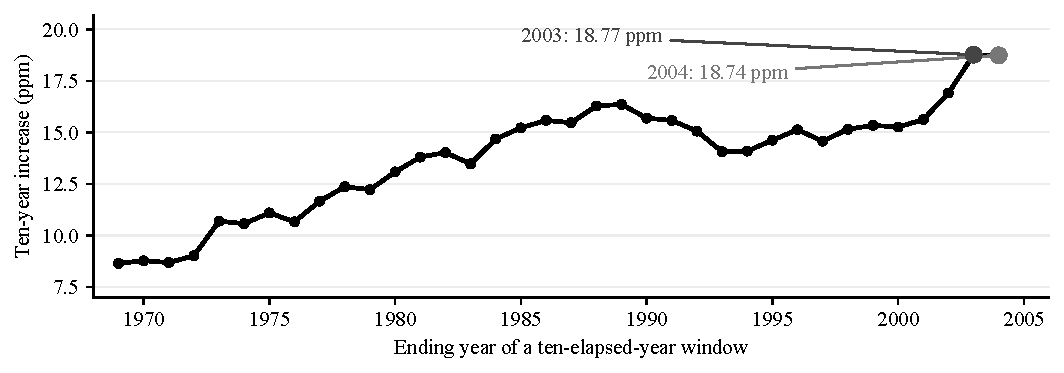
\includegraphics[width=.94\linewidth]{F01-r01.pdf}
\caption{\txt{FC01}{Supported annual ten-year changes from the supplied observations. The windows ending in 2003 and 2004 are nearly equal~\cite{workbook}.}}\label{fig:decade}
\end{figure}
\section{Concentration models}\label{sec:co2}
\p{CO201}{We use three deliberately simple continuations. They differ in what they hold constant: recent absolute growth, acceleration, or proportional growth. Let $x=(t-1959)/10$ and let the reference concentration be 315.98 ppm. One unit of $x$ is a decade. Least-squares fits use a stable singular-value-decomposition solution, with full stored precision retained for forecasts and threshold searches. The coefficients displayed below are rounded.}
\subsection{Recent absolute growth: D}
\p{CO202}{At forecast origin $o$, the recent-growth rule anchors to the latest concentration and continues the average annual increase over the preceding ten years. Its general form is}
\begin{equation}\label{eq:drift}
\widehat C_D(t\mid o)=C_o+s_o(t-o),\qquad s_o=\frac{C_o-C_{o-10}}{10}.
\end{equation}
\p{CO203}{Using the 2011 and 2021 endpoints gives the production path}
\begin{equation}\label{eq:drift-production}
\widehat C_D(t\mid 2021)=416.45+2.46(t-2021).
\end{equation}
\p{CO204}{This rule is easy to interpret and responds to recent growth. It does not attempt to explain the entire history with one fitted line, and its reliance on two endpoints can make an unusual recent interval influential.}
\subsection{Constant acceleration: Q}
\p{CO205}{The quadratic model fits concentration to a constant, $x$ and $x^2$ over the available training years. Its full-history production fit is}
\begin{equation}\label{eq:quadratic}
\widehat C_Q(t)=315.521509+8.057027x+1.303764x^2.
\end{equation}
\p{CO206}{Curvature allows the absolute increase to change with time. We do not constrain the quadratic coefficient to force acceleration, so turning points and nonpositive extrapolations must be checked rather than ruled out by assumption.}
\subsection{Proportional growth: E}
\p{CO207}{The exponential model fits the logarithm of concentration relative to 315.98 ppm as a linear function of $x$. Its production expression is}
\begin{equation}\label{eq:exponential}
\widehat C_E(t)=315.98\exp(-0.019627123+0.044917135x).
\end{equation}
\p{CO208}{This formulation holds proportional stock growth constant. Estimation minimizes squared errors in log units, but predictive comparisons use ppm for every concentration model. We assume neither a lognormal error distribution nor a mean correction on exponentiation. The equation is an empirical continuation, not an emissions-and-sinks mechanism.}
\subsection{Historical fit and residual behavior}
\begin{table}[H]\centering\small
\caption{\txt{TC03}{Production fit diagnostics, with the unequal fitting samples retained explicitly.}}\label{tab:fit}
\begin{tabular}{llrrr}\toprule
Path & Fit years & Observations & RMSE (ppm) & Lag-one residual correlation\\\midrule
D & 2011--2021 & 11 & 0.301 & 0.015\\
Q & 1959--2021 & 63 & 0.720 & 0.814\\
E & 1959--2021 & 63 & 2.888 & 0.979\\\bottomrule
\end{tabular}
\end{table}
\p{CO209}{Q follows the historical curve more closely than E, but both retain persistent residual patterns. D's smaller fit error covers only 11 observations and cannot fairly be ranked against the 63-point errors as though the samples matched. For that reason, the choice of a primary rule rests on forecasts made from earlier origins.}
\section{Comparing forecast accuracy}\label{sec:validation}
\p{VAL01}{For development, each rule is fitted using observations available through 1981, 1986, 1991, 1996 and 2001, then predicts the following one to ten years. The five-year spacing supplies several historical starting conditions while retaining a ten-year forecast task at every origin. These choices, including D's ten-year growth window, are declared design settings rather than settings shown to be optimal. The resulting 50 origin--horizon pairs end no later than 2011.}
\p{VAL02}{We select the concentration rule with the smallest pooled mean absolute error (MAE). Because MAE reports average absolute error in ppm, it puts all three models on the scale of the measured quantity without squaring large misses. Every forecast task receives equal weight, so a target year appearing at several origins receives more representation than one appearing only once. Root mean squared error (RMSE) and signed errors provide additional diagnostics. Writing the forecast error as $e_i$, the two summaries are}
\begin{equation}\label{eq:errors}
\operatorname{MAE}=\frac{1}{N}\sum_{i=1}^{N}|e_i|,\qquad
\operatorname{RMSE}=\sqrt{\frac{1}{N}\sum_{i=1}^{N}e_i^2}.
\end{equation}
\p{VAL03}{Numerical ties follow the declared order D, E, Q. After development selection, a fit ending in 2011 is assessed against 2012--2021 without intermediate refitting. The local computation preserves this order, but another reviewer had already exposed the final-period scores before the primary selection receipt. This is a later historical assessment, not a globally blind holdout.}
\begin{table}[H]\centering\small
\caption{\txt{TC04}{Concentration forecast errors in ppm for the declared development and later assessment tasks.}}\label{tab:co2-errors}
\begin{tabular}{lrrr}\toprule
Rule & Development MAE & Final MAE & Final RMSE\\\midrule
D & 1.48122 & 2.14450 & 2.52491\\
Q & 1.75903 & 1.39841 & 1.64292\\
E & 3.78876 & 8.24177 & 8.58429\\\bottomrule
\end{tabular}
\end{table}
\p{VAL04}{D wins the pooled development comparison. Q is the most accurate of the three on the later 2012--2021 assessment, with both lower MAE and lower RMSE than D. The distinction matters: preserving the earlier selection permits an honest assessment of its performance, whereas replacing it after seeing these errors would answer a different question. Neither result establishes the best future rule.}
\begin{figure}[H]\centering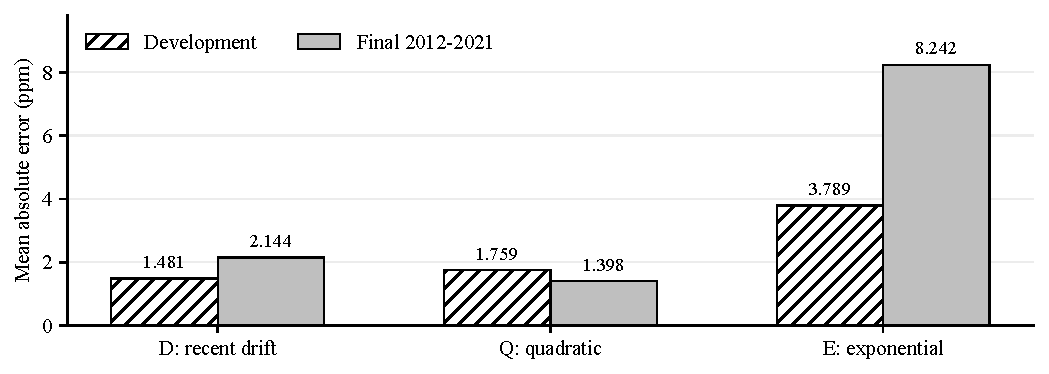
\includegraphics[width=.94\linewidth]{F02-r01.pdf}
\caption{\txt{FC02}{The D-versus-Q ranking reverses in the later assessment. Each final forecast originates in 2011 and is evaluated without intermediate refitting.}}\label{fig:ranking}
\end{figure}
\p{VAL05}{The pooled ranking also hides variation among origins. Q wins three development origins, D wins two, and omitting either 1986 or 1991 changes the pooled diagnostic winner to Q. These rank summaries were introduced after adversarial assessment and do not replace the original selector. D underpredicts every final concentration observation, with a ten-year error of $-4.07$ ppm. This pattern gives a concrete reason to question the persistence of its recent-growth assumption.}
\p{VAL06}{A post-assessment diagnostic asks whether the aggregation choice affects the ranking. It first averages absolute errors within each of the 30 target years, then gives those years equal weight. The resulting MAEs are 1.61035 ppm for D, 1.52284 ppm for Q and 3.94448 ppm for E, so Q now has the lowest score. This uses the same forecasts under a different loss rather than providing new validation. Both objectives are coherent for their stated purposes, and the original D selection remains unchanged.}
\section{Concentration projections and the 685-ppm exercise}\label{sec:projection}
\p{PRO01}{After the historical assessment, the unchanged rules are fitted through 2021 for production. Figure~\ref{fig:co2-paths} shows the resulting extensions alongside the supplied observations. Their divergence follows directly from the assumptions: D adds a constant amount each year, Q continues acceleration, and E compounds growth proportionally.}
\begin{figure}[H]\centering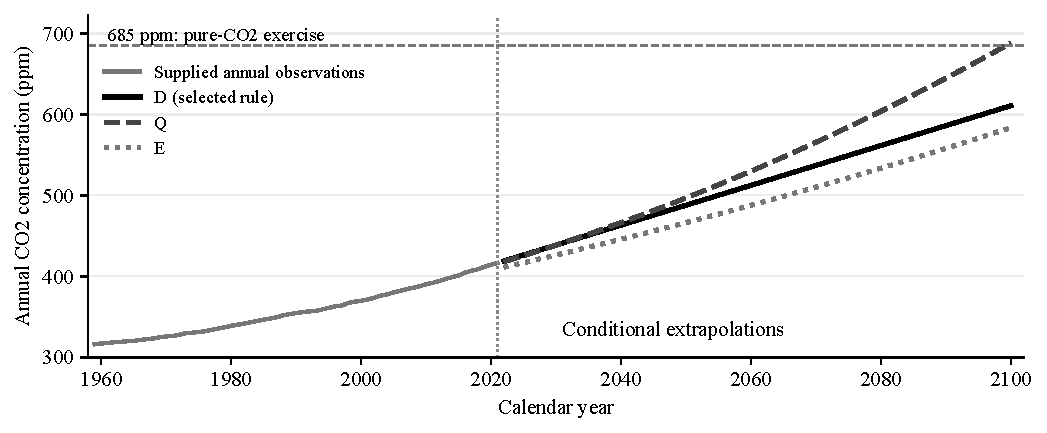
\includegraphics[width=.94\linewidth]{F03-r01.pdf}
\caption{\txt{FC03}{Conditional concentration paths through 2100. Observations end in 2021, and the horizontal reference is the requested pure-\CO{} threshold rather than OECD \CO{}-equivalent.}}\label{fig:co2-paths}
\end{figure}
\begin{table}[H]\centering\small
\caption{\txt{TC05}{All concentration candidates in the required future comparison.}}\label{tab:co2-future}
\begin{tabular}{lrrrr}\toprule
Path & 2050 (ppm) & 2050 minus 685 & 2100 (ppm) & First 685-ppm year\\\midrule
D & 487.79 & $-197.21$ & 610.79 & 2131\\
Q & 496.81 & $-188.19$ & 688.33 & 2100\\
E & 466.29 & $-218.71$ & 583.70 & 2136\\\bottomrule
\end{tabular}
\end{table}
\p{PRO02}{None reaches 685 ppm by 2050. Q first reaches it in 2100, followed by D in 2131 and E in 2136. We search integer annual values through 2300 and use unrounded values for the crossing decision. For D, the last value below and first value above are 684.59 and 687.05 ppm in 2130 and 2131. The corresponding pairs are 683.85754 and 688.32682 ppm for Q in 2099 and 2100, and 683.06729 and 686.14233 ppm for E in 2135 and 2136.}
\p{PRO03}{The spread between the three paths increases from 30.52 ppm in 2050 to 104.63 ppm in 2100. This is a comparison of assumptions, not a probability interval or an exhaustive bound on possible futures. Since the historical tests cover no more than ten years ahead, they cannot validate these much longer extrapolations. The reported digits preserve model arithmetic rather than imply comparable precision in future measurements.}
\section{A linked temperature forecast}\label{sec:temperature}
\p{TEM01}{We next ask whether concentration can be used in a simple temperature extension. Temperature is represented by an anomaly relative to 1951--1980 throughout. A full-history linear trend in time, T0, provides a baseline against which to compare the descriptive log-concentration relationship T1. Fitting through 2021 gives}
\begin{align}
\widehat T_0(t)&=-0.170257937+0.168183564x,\label{eq:t0}\\
\widehat T_1(C)&=-0.100573219+3.776119820\log(C/315.98).\label{eq:t1}
\end{align}
\p{TEM02}{The log form associates equal proportional concentration changes with equal changes in fitted anomaly. It offers a compact way to link the two series, but its slope is a descriptive coefficient rather than an identified climate sensitivity or policy effect. A comparison with T0 asks whether this particular linked construction improves on the specified linear-time baseline. It does not test every possible representation of time.}
\subsection{Evaluate the full forecasting chain}
\p{TEM03}{At each origin, T1 is fitted to the observed concentration--temperature pairs available by that date. Future temperature then uses forecast concentration from D, Q or E. Substituting realized future concentration would remove part of the actual forecast difficulty, so it is excluded from all scores. With fitted coefficients denoted by $\alpha_o$ and $\beta_o$, the linked forecast is}
\begin{equation}\label{eq:linked}
\widehat T_{1,m}(t\mid o)=\alpha_o+\beta_o\log\!\left(\frac{\widehat C_m(t\mid o)}{315.98}\right),\qquad m\in\{D,Q,E\}.
\end{equation}
\p{TEM04}{The selection is sequential. We first choose a concentration rule, then compare its linked temperature forecast with T0. This assesses the downstream consequence of the chosen concentration model rather than searching jointly for the smallest temperature error. The other linked paths remain visible as comparators.}
\begin{table}[H]\centering\small
\caption{\txt{TC06}{Temperature forecast errors and eligibility in the original sequential selection.}}\label{tab:temp-errors}
\begin{tabular}{lrrl}\toprule
Path & Development MAE (\degC) & Final MAE (\degC) & Selection role\\\midrule
T0 & 0.100011 & 0.124803 & Eligible\\
T1-D & 0.087214 & 0.093147 & Selected\\
T1-Q & 0.083687 & 0.090526 & Comparator\\
T1-E & 0.095634 & 0.121659 & Comparator\\\bottomrule
\end{tabular}
\end{table}
\p{TEM05}{T1-D improves on T0 in both periods and wins the eligible comparison. Yet T1-Q has slightly lower errors among all declared paths. Calling T1-D the global minimum would therefore misrepresent the results. There is a further reason for caution about unique concentration information: substituting exponential E into the logarithmic relationship produces a straight line in future time, although its calibration differs from T0.}
\subsection{Temperature thresholds}
\begin{figure}[H]\centering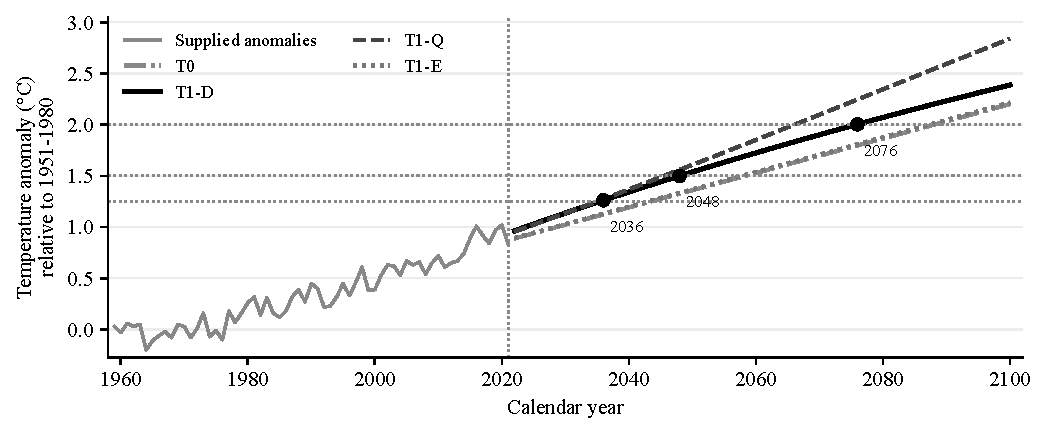
\includegraphics[width=.94\linewidth]{F04-r01.pdf}
\caption{\txt{FC04}{Temperature extensions relative to the 1951--1980 mean. Markers identify the selected T1-D annual threshold crossings, all beyond the ten-year tested horizon from 2021.}}\label{fig:temperature}
\end{figure}
\begin{table}[H]\centering\small
\caption{\txt{TC07}{Conditional crossing years and temperature anomalies for every declared path.}}\label{tab:temp-future}
\begin{tabular}{lrrrrr}\toprule
Path & 1.25\degC{} year & 1.50\degC{} year & 2.00\degC{} year & 2050 (\degC) & 2100 (\degC)\\\midrule
T1-D & 2036 & 2048 & 2076 & 1.54 & 2.39\\
T0 & 2044 & 2059 & 2089 & 1.36 & 2.20\\
T1-Q & 2035 & 2046 & 2067 & 1.61 & 2.84\\
T1-E & 2043 & 2058 & 2088 & 1.37 & 2.22\\\bottomrule
\end{tabular}
\end{table}
\p{TEM06}{The selected answer to the three requested thresholds is 2036, 2048 and 2076, conditional on T1-D's continuation. Here a crossing means the first integer year after 2021 whose unrounded central path reaches the specified level. It is neither the first realized warm year nor the start of sustained warming. Every value is relative to 1951--1980, so these dates must not be read as Paris-target or pre-industrial warming dates.}
\p{TEM07}{Rounding can otherwise change the apparent boundary. T0 gives 1.999310\degC{} in 2088, which displays as 2.00\degC{} but remains below the threshold. Its first crossing is correctly recorded as 2089. Table~\ref{tab:temp-future} also shows that changing the concentration assumption moves the linked dates, even when the same fitted temperature relationship is retained.}
\section{What the observed association does and does not show}\label{sec:relationship}
\p{REL01}{Concentration and temperature rise together strongly over 1959--2021. Their level correlation is 0.961318, while the correlation between log concentration and anomaly is 0.960366. The fitted log relationship has a descriptive coefficient of determination of 0.922302. That value describes variation accounted for by the fitted curve within this sample, not a percentage of warming caused by \CO{}.}
\begin{figure}[H]\centering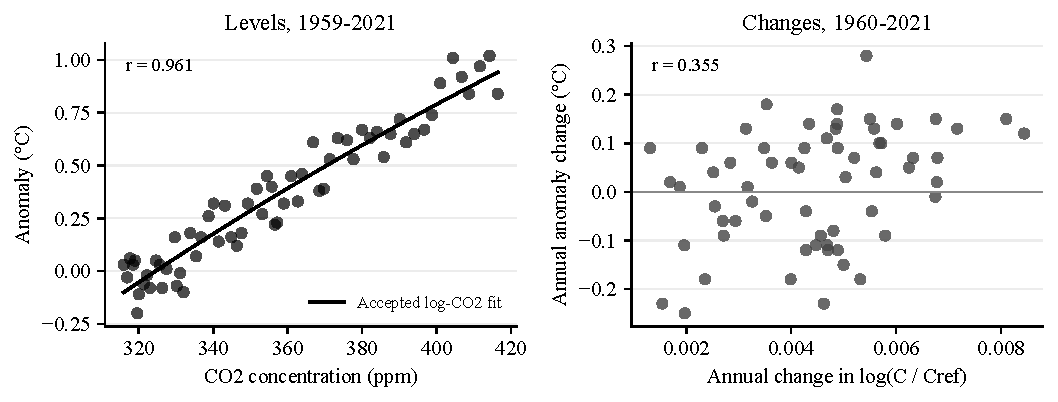
\includegraphics[width=.94\linewidth]{F05-r01.pdf}
\caption{\txt{FC05}{Levels and annual changes answer different descriptive questions. The left panel includes the accepted log-concentration fit, while the right uses changes read from the accepted diagnostic series.}}\label{fig:association}
\end{figure}
\begin{table}[H]\centering\small
\caption{\txt{TC08}{Association diagnostics using the full primary period.}}\label{tab:association}
\begin{tabular}{p{.51\linewidth}lrr}\toprule
Diagnostic & Years & Pairs & Correlation\\\midrule
\CO{} level and anomaly & 1959--2021 & 63 & 0.961318\\
Log-\CO{} level and anomaly & 1959--2021 & 63 & 0.960366\\
Log-\CO{} and anomaly after linear time detrending & 1959--2021 & 63 & 0.551057\\
Log-\CO{} and anomaly after quadratic time detrending & 1959--2021 & 63 & 0.491659\\
Annual changes in log-\CO{} and anomaly & 1960--2021 & 62 & 0.355269\\\bottomrule
\end{tabular}
\end{table}
\p{REL02}{Removing separate linear or quadratic time trends weakens the association, and examining annual changes weakens it further. The contrast is visible in Figure~\ref{fig:association}. Detrending and differencing remove low-frequency information and change the question being asked, so weaker correlations neither disprove a physical greenhouse mechanism nor identify its magnitude.}
\p{REL03}{These records omit other forcings, response delays and relevant drivers. Serial dependence and the pairing of a station indicator with a global temperature index add further limits. We therefore interpret the relationship descriptively, without independent-observation significance tests or an estimate of causal climate sensitivity.}
\section{Forecast horizons, observed failures and sensitivity}\label{sec:reliability}
\subsection{What the historical tests establish}
\p{HOR01}{The tests give comparative error evidence for the declared rules at horizons of one to ten years. They do not identify a universal date at which a forecast becomes unreliable. Table~\ref{tab:horizons} reports selected horizons, with final errors belonging to forecasts made in 2011 and checked against 2012, 2016 and 2021. These are not observed errors in 2022, 2026 or 2031.}
\begin{table}[H]\centering\small
\caption{\txt{TC09}{Selected horizon evidence for the retained D and T1-D pipeline.}}\label{tab:horizons}
\begin{tabular}{r r r r r}\toprule
Horizon & D development & D final absolute & T1-D development & T1-D final absolute\\
(years) & MAE (ppm) & error (ppm) & MAE (\degC) & error (\degC)\\\midrule
1 & 0.36420 & 0.15700 & 0.093956 & 0.062471\\
5 & 1.12300 & 2.29500 & 0.084078 & 0.222292\\
10 & 2.28000 & 4.07000 & 0.053046 & 0.039622\\\bottomrule
\end{tabular}
\end{table}
\p{HOR02}{There are five development origins per horizon, but the 50 forecast pairs cover only 30 distinct target years. The overlapping tasks and the ten final observations cannot be treated as independent trials. Applying the same ten-year maximum from 2021 gives a display cutoff of 2031, not a validated reliability date. Continued use requires reassessment as observations arrive.}
\subsection{A historical error reference and its miss}
\p{ENV01}{For a simple reference around the selected forecast, we take the largest absolute development error seen across all origins and all horizons no greater than the horizon of interest. With development origins denoted by $\mathcal O$, the radius is}
\begin{equation}\label{eq:envelope}
B_h=\max_{o\in\mathcal O,\,1\leq j\leq h}|e_{o,j}|.
\end{equation}
\p{ENV02}{This construction gives a nondecreasing historical error radius. It is fixed before the later assessment and is not calibrated as a confidence or prediction interval. Figure~\ref{fig:envelope} shows what happens when the reference is confronted with the later observations.}
\begin{figure}[H]\centering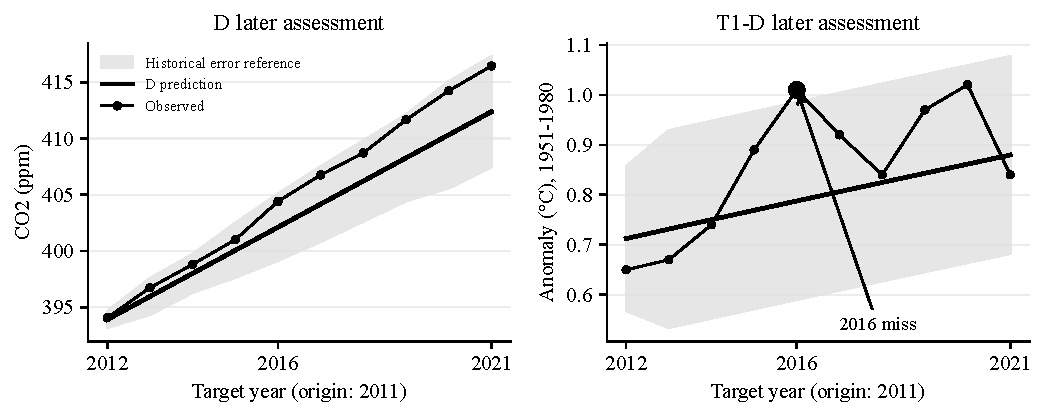
\includegraphics[width=.94\linewidth]{F06-r01.pdf}
\caption{\txt{FC06}{Fixed development-derived error references on forecasts from 2011. The T1-D reference misses the 2016 observation, and the shaded regions do not imply a future coverage probability.}}\label{fig:envelope}
\end{figure}
\begin{table}[H]\centering\small
\caption{\txt{TC10}{The 2016 temperature miss in the selected T1-D forecast.}}\label{tab:miss}
\begin{tabular}{lr}\toprule
Quantity & Value (\degC)\\\midrule
Predicted anomaly & 0.787708\\
Observed anomaly & 1.010000\\
Absolute error & 0.222292\\
Historical radius at horizon 5 & 0.197125\\
Excess beyond radius & 0.025167\\\bottomrule
\end{tabular}
\end{table}
\p{ENV03}{D's reference contains all ten later concentration observations, whereas T1-D's contains nine of the ten temperatures. In 2016, the absolute temperature error exceeds the radius by 0.025167\degC{}. We retain the original radius and the miss. Nine contained observations out of ten temporally related checks do not estimate 90\% future coverage, and the actual miss rules out treating this reference as a guaranteed bound.}
\subsection{Changing the fitting window and model form}
\p{SEN01}{The declared window sensitivity refits the selected forms using the last 30 observations, 1992--2021. D is unchanged because it still uses the same last-ten-year increase. That invariance follows from its definition, rather than demonstrating that the whole forecasting chain is insensitive to history. Refitting the temperature association changes both future anomalies and crossing dates.}
\begin{table}[H]\centering\small
\caption{\txt{TC11}{Sensitivity of T1-D to its fitting period.}}\label{tab:window}
\begin{tabular}{lrr}\toprule
Quantity & Full history & Last 30 observations\\\midrule
2050 anomaly (\degC) & 1.53904 & 1.64488\\
2100 anomaly (\degC) & 2.38817 & 2.59910\\
First 1.25\degC{} year & 2036 & 2033\\
First 1.50\degC{} year & 2048 & 2044\\
First 2.00\degC{} year & 2076 & 2068\\\bottomrule
\end{tabular}
\end{table}
\p{SEN02}{The three dates move 3, 4 and 8 years earlier. Changing the model form matters too: the linked 2100 anomalies span 2.21685--2.83946\degC{}, or 2.20113--2.83946\degC{} when T0 is included. These comparisons retain the original selector and quantify sensitivity to specified alternatives. They are not a new optimized model or probability bounds.}
\section{Model appraisal}\label{sec:appraisal}
\p{APP01}{The framework's main strength is that its assumptions are visible. Each concentration model has few parameters, historical forecasts respect the observations available at their origin, and temperature scores include upstream concentration forecast error. Comparing different forms also reveals an uncertainty that a single fitted curve would hide. This transparency makes the analysis inspectable, even where its conclusions are limited.}
\p{APP02}{The same simplicity restricts the model. D assumes recent growth persists, Q lets curvature dominate distant behavior, and E describes proportional stock growth without an emissions-and-sinks balance. T1 omits response delays and other drivers. More elaborate curves would add flexibility, but the short record of evaluated horizons would still provide little evidence about their century-scale behavior. A logistic capacity is not identified by the rising record, and a physical carbon-cycle or energy-balance model would require inputs absent from the two supplied series.}
\subsection{Calculation validity}
\p{APP03}{All actual full-history and declared last-30-observation paths are finite, valid and nondecreasing over the annual search domain 2021--2300. Their reported crossing boundaries satisfy the unrounded comparisons, and the supplied history does not exceed the requested levels. These checks establish that the calculations have the stated mathematical status. They do not establish climate credibility through 2300.}
\p{APP04}{A first-passage search uses only the contiguous valid portion of a path from its origin. A crossing before a later invalid value is retained with a warning, while invalidity before any crossing blocks a date. Already-above-origin and valid non-crossing-through-2300 cases receive different statuses. A later valid segment cannot bridge an invalid gap. None of the actual primary paths requires such a rescue.}
\section{Conclusions}\label{sec:conclusion}
\p{CON01}{The historical claim has a narrow but clear answer. In the supplied annual series, the ten-year increase ending in 2004 is second to the one ending in 2003. The difference is only 0.03 ppm, and it does not settle a March-specific assertion. Source definitions remain just as consequential in the future comparison: our pure-\CO{} calculations and OECD's \CO{}-equivalent benchmark describe different quantities.}
\p{CON02}{For the stated concentration models, the 2100 projections range from 583.70 to 688.33 ppm. None reaches 685 ppm by 2050. The selected temperature path reaches 1.25, 1.50 and 2.00\degC{} above 1951--1980 in 2036, 2048 and 2076, conditional on its continuation. Those answers are useful as consequences of explicit assumptions. Their precision should not obscure how readily other assumptions move them.}
\p{CON03}{The tests explain why that distinction is necessary. D wins the declared pooled development comparison, yet Q does better in the later period. T1-Q also slightly outperforms the selected T1-D path, whose historical error reference misses 2016. Refitting the temperature relationship over a shorter window moves the requested crossings several years earlier. Taken together, these results support comparison and reassessment rather than confidence in one distant trajectory.}
\p{CON04}{Historical testing still contributes evidence. It describes relative errors for specified rules over one- to ten-year tasks and exposes weaknesses that an in-sample fit would miss. It does not supply a universal expiry date for the model. Keeping definitions consistent, monitoring errors and comparing alternative assumptions are therefore practical consequences of this analysis. Quantifying a particular intervention's benefit would require emissions, forcing and response evidence beyond these two records.}
\clearpage
\section{Article for Scientific Today}\label{sec:article}
\begin{center}{\large\bfseries Climate numbers need more than a date}\end{center}
\p{ART01}{A concentration figure can be accurate yet answer the wrong question. We examined the records supplied through 2021 for a mathematical modeling exercise, beginning with what each number measures.}
\p{ART02}{The supplied carbon dioxide values are annual Mauna Loa averages, despite the question's reference to March. Their ten-year rise ending in 2004 was 18.74 parts per million, just below 18.77 ppm ending in 2003. That small difference does not settle the separate March claim. NOAA's source supports about 421 ppm for the monthly average in May 2022, a later observation that we excluded from our fitted models~\cite{problem,workbook,noaa-data,noaa-news}.}
\p{ART03}{Three simple extensions of past concentration changes produce roughly 466--497 ppm in 2050 and 584--688 ppm in 2100. None reaches 685 ppm by 2050. This does not refute OECD, whose cited figure combines greenhouse gases as \CO{}-equivalent rather than measuring \CO{} alone~\cite{oecd}.}
\p{ART04}{Model choice changes the answer. A recent-growth rule performed best in the planned development comparison, but a quadratic curve did better on the later 2012--2021 assessment. Neither has demonstrated universal superiority. We retain the original selection instead of choosing again after seeing those errors.}
\p{ART05}{Our selected temperature path, driven by the recent-growth concentration rule, reaches 1.25, 1.50 and 2.00\degC{} above the 1951--1980 average in 2036, 2048 and 2076. Driving the same relationship with the quadratic concentration path gives slightly smaller errors. Other models and fitting periods move the dates. They describe conditional annual paths, not established deadlines, sustained warming dates or Paris targets. The observed association does not isolate cause either.}
\p{ART06}{The tests extend only ten years ahead, and a range based on earlier temperature errors missed the 2016 observation. There is no guaranteed reliability date or established probability attached to a century-scale projection. Continued measurement and regular comparison with observations matter more than treating a calculated date as certain. Planning can compare several assumptions, while evaluating interventions also requires evidence on emissions, other climate drivers and response delays.}
\clearpage
\addcontentsline{toc}{section}{References}
\begin{thebibliography}{9}
\bibitem{problem}\txt{REF01}{COMAP. \emph{2022 HiMCM Problem B: \CO{} and Global Warming}. 2022. Official four-page statement supplied in the local archive. Requirements appear on page 1, delivery rules on page 2, and data with source notes on pages 3--4.}
\bibitem{workbook}\txt{REF02}{COMAP. \emph{2022\_HiMCM\_Data.xlsx}. 2022. Supplied \CO{} Data Set 1 and Temps Data Set 2. This workbook is the sole numerical modeling input, with source hashes retained in the companion project.}
\bibitem{noaa-data}\txt{REF03}{NOAA Global Monitoring Laboratory and Scripps Institution of Oceanography. \emph{Trends in Atmospheric Carbon Dioxide}. Annual and monthly Mauna Loa data definitions. Definition snapshots inspected on 3 November 2026, with current observations excluded from modeling. \href{https://gml.noaa.gov/ccgg/trends/data.html}{Official data documentation}.}
\bibitem{noaa-news}\txt{REF04}{NOAA. \emph{Carbon dioxide now more than 50\% higher than pre-industrial levels}. 3 June 2022. Monthly May concentration and site context. \href{https://www.noaa.gov/news-release/carbon-dioxide-now-more-than-50-higher-than-pre-industrial-levels}{Official news release}.}
\bibitem{nasa}\txt{REF05}{NASA Goddard Institute for Space Studies. \emph{GISTEMP Frequently Asked Questions}. Anomaly baseline and land-ocean temperature index definitions, inspected on 3 November 2026. \href{https://data.giss.nasa.gov/gistemp/faq/}{Official FAQ}.}
\bibitem{oecd}\txt{REF06}{OECD. \emph{OECD Environmental Outlook to 2050: The Consequences of Inaction}. OECD Publishing, 2012. Chapter 3, especially printed page 83, and the baseline scenario definition. Primary report text was inspected, with selected evidence retained as a labeled excerpt and paraphrase rather than an original downloaded PDF. \href{https://www.oecd.org/content/dam/oecd/en/publications/reports/2012/03/oecd-environmental-outlook-to-2050_g1g14e69/9789264122246-en.pdf}{Official report}.}
\end{thebibliography}
\section*{Practice, AI use and reproducibility}
\addcontentsline{toc}{section}{Practice, AI use and reproducibility}
\p{DIS01}{This is a retrospective practice exercise, not a live entry or external submission. Codex collaboration sessions carried out coordination, source admission, modeling, computation, writing, visualization and independent review, with some roles operating sequentially. The user delegated reversible practice decisions to the coordinator. No human checkpoint response or Claude Code execution is invented.}
\p{DIS02}{The report uses the accepted scientific run T05-scientific-20261103-r03 and its scoped claim register. Source versions, commands, fixed numerical outputs and evidence bindings remain in the companion project. Figures display accepted tables without refitting. Independent numerical review is distinct from writer checks of the exported PDF and from independent review of this revised artifact.}
\p{DIS03}{Candidate forms and the selector were fixed before adversarial final-score exposure. The local primary run retained selection before final scoring, but prior project-wide access means there was no globally unseen holdout. Later interpretation and implementation safeguards are post-exposure repairs. Earlier failures and repaired artifacts are preserved.}
\p{DIS04}{The producer reports 44 implementation tests and byte-identical reproduction of 32 numerical outputs from 88 recovered dependencies. These establish execution and reproducibility evidence rather than future scientific accuracy. The additional target-year weighting comparison is a separately reviewed post-assessment diagnostic and does not alter the original selection.}
\p{DIS05}{This manuscript is authored in LaTeX and compiled with XeLaTeX. Text, headings, tables, captions and plot labels use the installed Times New Roman family. Mathematical notation uses the Times-compatible NewTX math fonts for symbols and layout that the text family does not supply. Font files are referenced from the local installation and are not distributed with the source.}
\end{document}
